\section{Architecture and Implementation}\label{sec:Architecture}
% Describe the data processing pipeline here. 
% 1. Get the raw data and remove the ground (LiDAR data clean up)
% 2. Segment data and sent it to classifier 
% 3. Classification with Neural Network. 

Our data processing pipeline consist of 3 main processing steps: 

\begin{enumerate}
  \item \textbf{Step-1 Data Filtering. } Filtering the LiDAR base lines (cylinder lines around objects - See Figures \ref{fig:ground_before} and \ref{fig:after})
  
  \item \textbf{Step-2 Object Segmentation.} Separating the 3D point cloud to segments that contain one single object or in other words marking the object with a voxel grid.
    
  \item \textbf{Step-3 Object Classification.}  Classifying an object from point cloud data containing one single object.
\end{enumerate}

\begin{figure*}[!h]
 \begin{center}
   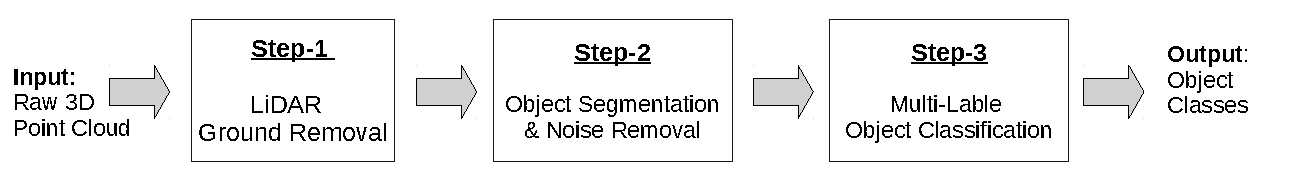
\includegraphics[width=0.9\textwidth]{./images/DataProcessingPipleline.pdf}
   \caption{Overview of our Data Processing Pipeline}
   \label{fig:dataPipeline}
 \end{center}
\end{figure*}


Figure \ref{fig:dataPipeline} depicts our data processing pipeline. As the system runs in the testing it gets point cloud data for a single scene which includes multiple objects and process it in 3 steps and to deliver the classification results in real-time.   

The provided training data by DEBS 2019 Challenge \cite{DEBSGC2019} includes only one single object per scene with its label so that it is not require to have the step-2 object segmentation when we train our system.






% Describe \ldots. 
% 
% Different forms of data processing architectures that we have implemented and tested . 
% 
% \begin{enumerate}
%   \item Different methods for removing noise from raw data (data preprocessing). 
%   \item Projecting 3D data into 2D data using 3 different projection methods 
%   \item CNN  (with and without maxpool) + fully-connected + dropout + fully-connected+softmax
%   \item CNN with different number of hidden layers. 
% 
% \end{enumerate}



% KIA
% We need another image to describe the CNN architecture. 
% Add two images about it. 




\subsection{LiDAR Ground Data Removal}
% Describe here how we remove the ground - keep this very general 
% 

The first step in our data processing pipeline is to filter out the LiDAR laser lines that are building a cylinder form 3D shape from the laser standing point $(x=0, y=0, z=0)$. Figure \ref{fig:ground_before} visualizes the LiDAR data from a single scene with LiDAR laser lines and Figure \ref{fig:after} shows the data after filtering the Laser ground lines. As you can see objects like car or pedestrian are visible in Figure \ref{fig:after} after filtering the LiDAR lines.

This first filtering step in our data processing pipeline reduces highly the amount of data that we process and also helps to be able to find object segments in the next following step. 
We train and test the classification model (in the Step-3) after removing the Laser base lines and filtering them out.  


\begin{figure*}[!h]
\centering
\begin{minipage}{0.49\textwidth}
  \centering
        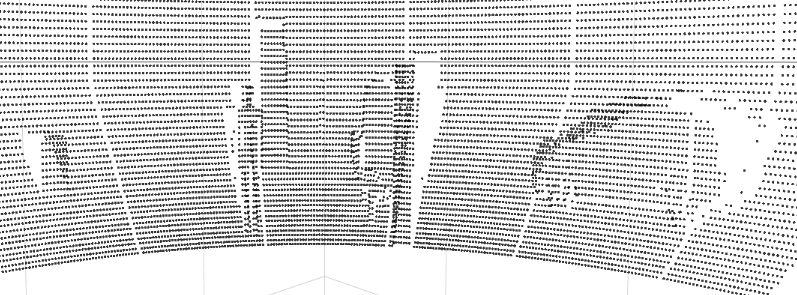
\includegraphics[width=.9\linewidth]{images/ground_before2.png}
        \caption{LiDAR Raw Point Cloud Data}
        \label{fig:ground_before}
\end{minipage}%
\begin{minipage}{0.49\textwidth}
  \centering
        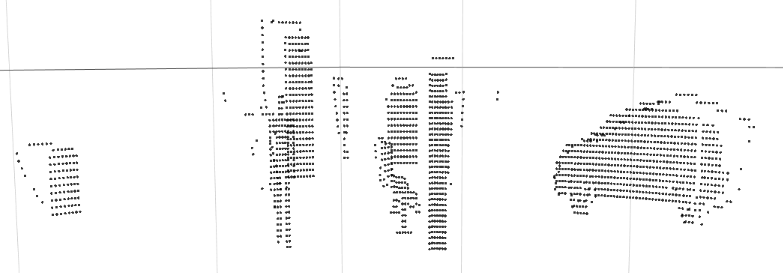
\includegraphics[width=.9\linewidth]{images/ground_after2.png}
        \caption{Data After Filtering the LiDAR Scan Lines}
        \label{fig:after}
\end{minipage}%
% \caption{General caption.} \label{fig:1}
\end{figure*}


% Describe here how we filter the ground. 



\subsection{Object Segmentation and Noise Removal}
The first during the testing phase is to segment the point cloud to chunks of data that include possibly only one single object.
For this task we have implemented different clustering methods to cluster the data in original 3 dimensional format and in projected 2D form.      



\textbf{3D to 2D Projection.} We have projected the 3D data in 4 different ways to 2D data. The first 3 methods is just to consider the data by dropping one of the axis, for examples by dropping the y axis and considering the x and z axis.  The last method was to project 3D data by using a point of eye view and project each data point to a plane (also named window) in a distance d.  The following formula gives us the new $(x',  y')$ after projecting the $(x,y,z)$ to a plane in distance d. 

% \large 
\begin{align*}
d  & = \text{Distance to a projection plane} \\   
x' & =  x (\frac{d}{z}) \\  
y' & =  y (\frac{d}{z}) \\
z' & =  z (\frac{d}{z}) = d  
\end{align*}
% \normalsize



\textbf{Object segmentation using Clustering.} We have implemented and tested the following clustering methods to build segments of point cloud that contain as well as possible only one single separated object.  

\begin{enumerate}
  \item \textbf{K-means and Minibatch-Kmeans} on the 3D and project 2D data.    
  \item \textbf{Meanshift} (on 3D and 2D data) 
  \item \textbf{DBSCAN}  (on 3D and 2D)
\end{enumerate}

\textbf{K-means Clustering.} We run multiple iterations of k-means with different batch sizes and also applied elbow method to determine the optimal number of clusters.
Our evaluation result (Sec \ref{sec:Evaluation}) showed that the k-means algorithm cannot separate the data into one-object segments with high quality. It also could not achieve real-time processing when we need to test different number of clusters. 

\textbf{Density based Clustering Approaches - Meanshift and DBSCAN.} We observed that density based approaches can build better object segments in comparison to K-Means clustering mainly because of two important factors, 1. Density of LiDAR points are approximately equal on different objects considering the fact that we have areas/spaces with and without objects. In the case that there is an object, the density of points are roughly equal independent of type of object 2. When objects are close to each other or hiding each other partially, density-based approaches can achieve better segments and does not joint the two different clusters of the two objects.  

We have evaluated the segmentation step with different parameters (density value and number of minimum samples in each cluster). We observed that the segments build based on 3D DBSCAN approach can achieve acceptable real-time performance and  DBSCAN can be build better quality segments in 3D than using the algorithm with projected 2D data. However, we also observed that the classification of object types in the following step can fail to recognize objects correctly because the segmentation quality is not sufficient. 


DBSCAN clustering algorithm is also able to remove the noise form the data set and return point cloud data with cluster labels. 


\begin{figure*}[!h]
\begin{center}
  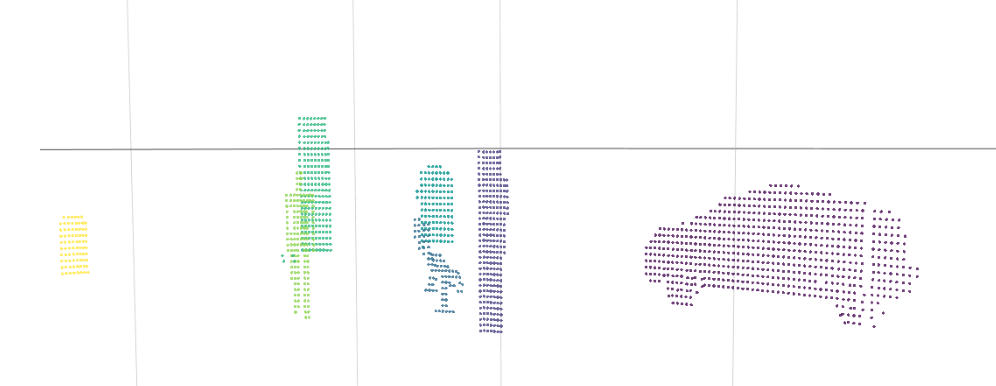
\includegraphics[width=.85\linewidth]{./images/seg_noise_removal.png}
  \caption{Clustered Point Cloud Data after Filtering the Data Noise (Colors indicate Clusters). }
  \label{fig:ClusteringWithNoiseFiltering}
\end{center}
\end{figure*}



\textbf{Sectioning From Top-View.}
To achieve better object segmentation, we developed a new approach by viewing the data from the top-view (considering data from the top elevation view (bird-view)) and projecting it to 2D. The LiDAR laser scanner is then positioned at the center point with the coordinate of (0, 0, 0), we can see that there are areas or spaces that are not occupied by any objects and there are sections with objects inside.     

Figure \ref{fig:sectors1} depicts the top-view of the LiDAR point cloud data. 
The red point is the zero point which is the position of the LiDAR scanner. All other surrounding points are object points from the top-view.  

Our idea for sectioning the data from top-view is illustrated in Figure \ref{fig:sectors2}. We calculate for each point the degree of angel that they have to the starting x-axis. As we know angles of points will be between 0 and 360 degrees. We sort the list of angles and see for which ranges of angles we have number of data points under a certain threshold (or we have no data). Then we can clearly separate the data into sectors by using the degree ranges that have no data points or less than a threshold. If the objects are very close to the LiDAR laser positron, then we might have data in all ranges of angel degrees, but we would then be able to separate the data by using a threshold.  


\begin{figure*}[!h]
\centering
\begin{minipage}{0.44\textwidth}
  \centering
         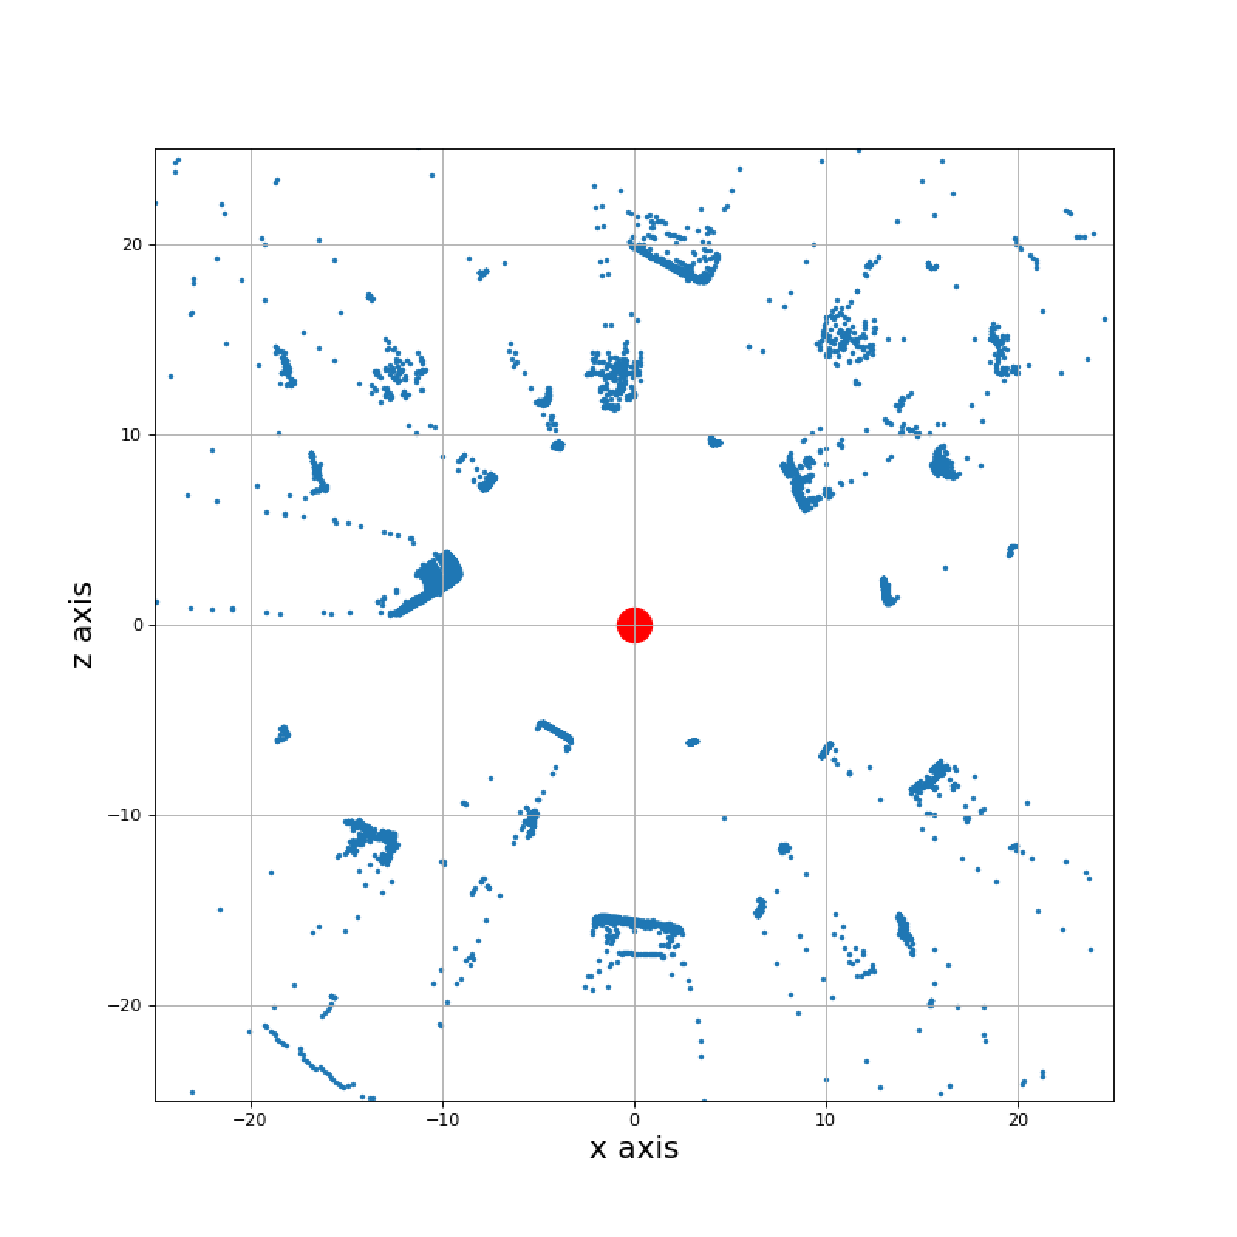
\includegraphics[scale=0.445]{./images/sector-transforms/scene-with-centre.pdf}
       \caption{Top-View of LiDAR Data}
       \label{fig:sectors1}
\end{minipage}%
\begin{minipage}{0.44\textwidth}
  \centering
        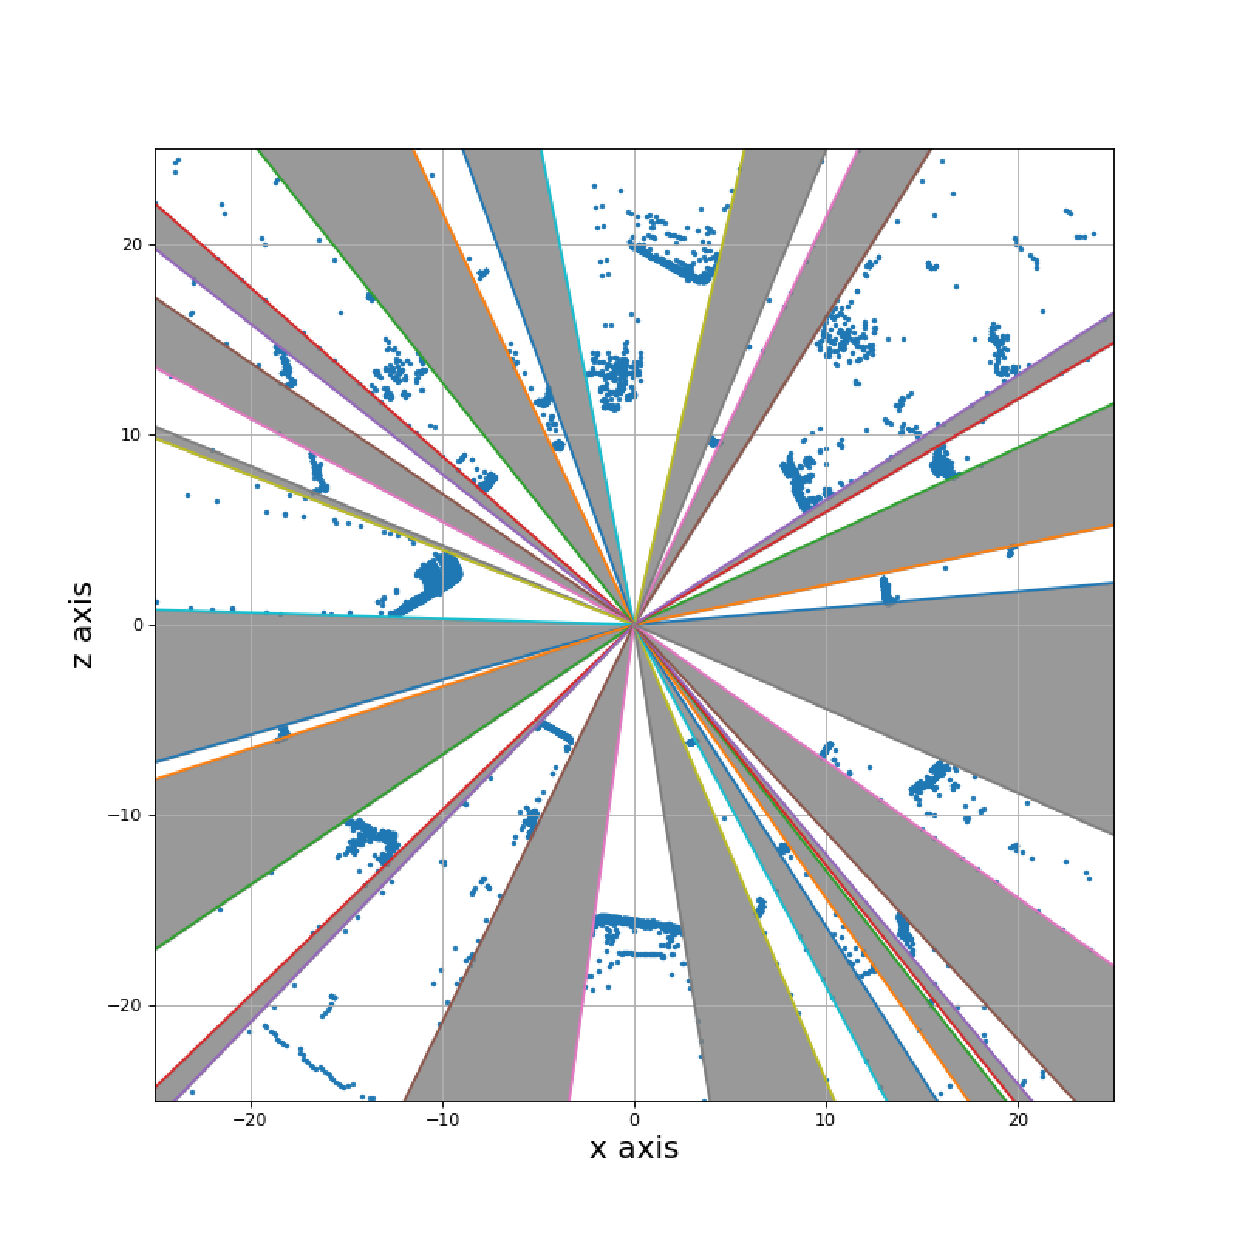
\includegraphics[scale=0.448]{./images/sector-transforms/scene-with-sector.pdf}
        \caption{Top-View - Separating unoccupied spaces/sectors (gray colored) from sectors with objects}
        \label{fig:sectors2}
\end{minipage}%
% \caption{General caption.} \label{fig:1}
\end{figure*}


The next step in object segmentation in this approach is to go into each sector and separate data in one sector into multiple sub-sectors.
For this purpose we calculate the radius of each point to the center ($\sqrt{x^2 + z^2 } $). Then we create the density of these radius values and separate the data from the local minimums.  An example of density curve is shown in Figure \ref{fig:SectorDensity} with the objects in a sector. If the density local minimum points of zero then, we can separate it from the zero points, and if local minimums are very close to each other and have large values then we need to send it to a clustering approach like DBSCAN for clustering.  

\begin{figure}[!h]
\begin{center}
  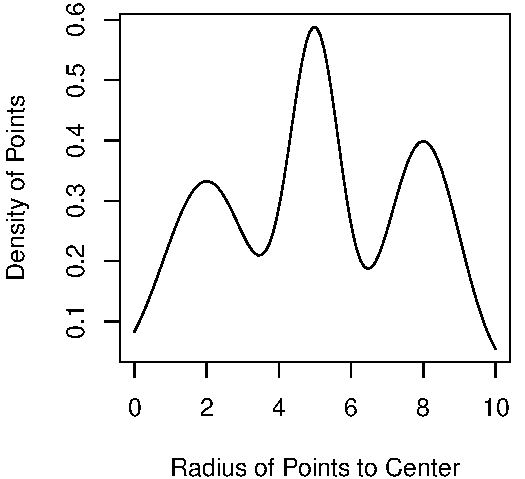
\includegraphics[scale=0.31]{./images/sectors_density.pdf}
  \caption{Density of Points in a Single Sector with 3 Objects}
  \label{fig:SectorDensity}
\end{center}
\end{figure}


Our evaluation contains segmentation with DBSCAN segmentation on 3D point cloud and on projected 2D data without Sectioning from top-view.  

